\begin{document}
\SweaveOpts{concordance=TRUE}


We want to predict the age of an abalone using its longest shell measurement and 
its weight.

See \url{https://archive.ics.uci.edu/ml/machine-learning-databases/abalone/} for more details.

\begin{knitrout}
\definecolor{shadecolor}{rgb}{0.969, 0.969, 0.969}\color{fgcolor}\begin{kframe}
\begin{alltt}
import pandas as pd

url = \hlstr{"https://archive.ics.uci.edu/ml/machine-learning-databases/abalone/abalone.data"}
abalone = \hlkwd{pd.read_csv}(url, sep=\hlstr{','}, 
                      names=[\hlstr{"sex"}, \hlstr{"longest_shell"}, \hlstr{"diameter"}, \hlstr{"height"}, \hlstr{"whole_weight"}, \hlstr{"shucked_weight"}, \hlstr{"visceral_weight"}, \hlstr{"shell_weight"}, \hlstr{"rings"}])

abalone = abalone[[\hlstr{'longest_shell'}, \hlstr{'whole_weight'}, \hlstr{'rings'}]]
\end{alltt}
\end{kframe}
\end{knitrout}

```{r engine='python'}
import pandas as pd
url = "https://archive.ics.uci.edu/ml/machine-learning-databases/abalone/abalone.data"
abalone = pd.read_csv(url, sep=',', names=["sex", "longest_shell", "diameter", "height", "whole_weight", "shucked_weight", "visceral_weight", "shell_weight", "rings"])

abalone = abalone[['longest_shell', 'whole_weight', 'rings']]
```

\begin{itemize}
  \item[a)] Plot \texttt{LongestShell} and \texttt{WholeWeight} on the $x$- 
  and $y$-axis, respectively, and color points according to \texttt{Rings}.
\end{itemize}

Using \texttt{mlr3}:

\begin{itemize}
  \item[b)] Create an \texttt{mlr3} task for the \texttt{abalone} data.
  \item[c)] Define a linear regression learner (for this you will need to load 
  the \texttt{mlr3learners} extension package first) and use it to train a 
  linear model on the \texttt{abalone} data. 
  \item[d)] Compare the fitted and observed targets visually. \\
  (Hint: use \texttt{autoplot()}.)
  \item[e)] Assess the model's training loss in terms of MAE. \\
  (Hint: losses are retrieved by calling \texttt{\$score()}, which accepts 
  different \texttt{mlr\_measures}, on the \\ prediction object.)
\end{itemize}

\vspace{1cm}
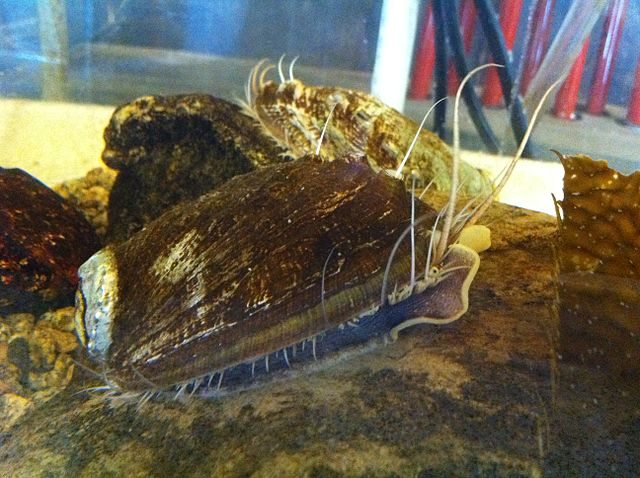
\includegraphics[width=0.5\textwidth]{figure/abalone}

\scriptsize{\url{https://en.wikipedia.org/wiki/Abalone#/media/File:LivingAbalone.JPG}}
\end{document}
